\begin{Exercise}[title=Indice d'un liquide]
Une cuve en verre a la forme d’un prisme de section droite rectangle isocèle. Elle est posée horizontalement sur une des arêtes de longueur $l$ du triangle isocèle, et le sommet opposé à ce côté est ouvert pour permettre de remplir la cuve d’un liquide transparent d’indice $n$.
Un pinceau de lumière est envoyé horizontale-
ment sur la face verticale de la cuve, dans un plan de section droite, à la hauteur $l/2$.
Ce rayon émerge au-delà de l’hypothénus et rencontre en un point $P$ un écran $E$ placé verticalement à la distance $l$ de la face d’entrée du dispositif.
On néglige l’effet dû aux parois en verre
sur la propagation du pinceau de lumière.
\Question Quelle limite supérieur peux on donner à la valeur de l'indice?
\Question Quel l'indice $n$ du liquide contenu dans la cuve e, fonction de $l$ et $z$
\Question Calculer $n$ avec $l=30 cm$ et$z=6.7cm$
\begin{center}
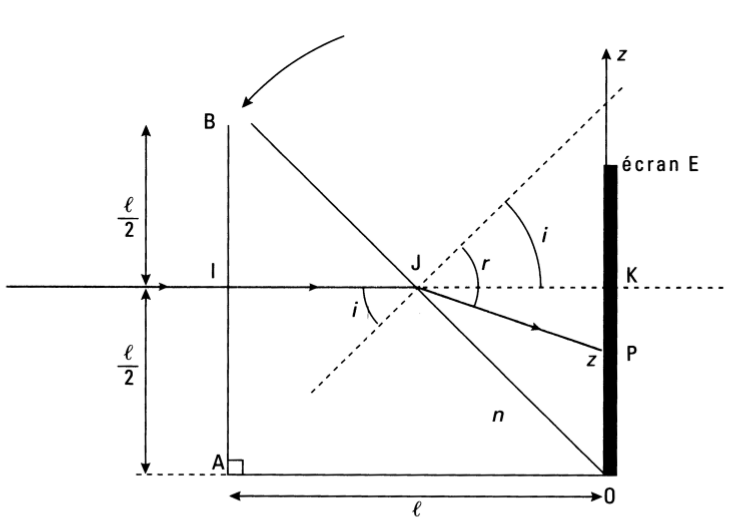
\includegraphics[scale=0.4]{./fig/indice_liq.png}
\end{center}
\end{Exercise}
\begin{Answer}
\Question $n\leq 1.414$
\Question $n =\sqrt{2}\sin\left(i+\arctan\left(\frac{l-2z}{l}\right)\right)$
\Question n=1.36 , ethanol?
\end{Answer}
